%######## IT 497 Assignment 2 #########
%Author - Gunjankumar Sharma
%######################################

%Before we start, I hope you have gone throught the README.md file.
%If not then please go through it.

%It is a pre-requisite to upload images as directed in the README file.

%Please read the comments which precede the line of code for a better understanding.


\documentclass[a4paper]{article}

%This is used to override the default behavior
%In this case, no size/scaling options will be passed to the \includegraphics{} directive and the height and width options will determine both the runtime generated graphic file sizes and the size of the graphics in your final document
%Reference - http://stat.ethz.ch/R-manual/R-devel/library/utils/html/RweaveLatex.html
\usepackage[nogin]{Sweave}

%This will add a frame to an input command in a code chunk 
\DefineVerbatimEnvironment{Sinput}{Verbatim} {xleftmargin=2em,xrightmargin=2em,
                                              frame=single}
%This will add a frame to the output of any command in a code chunk
\DefineVerbatimEnvironment{Soutput}{Verbatim}{xleftmargin=2em,xrightmargin=2em,
                                              frame=single}
%This package is used for aligning figures and tables 
\usepackage{float}
\textwidth=6.2in
\textheight=8.5in
\oddsidemargin=.1in
\evensidemargin=.1in
\headheight=-.2in

\begin{document}
\input{Assignment2-concordance}
\title { NBA Team Statistics - Chicago Bulls}
\author { Gunjankumar Sharma \\
\texttt{ gsharma@ilstu.edu}}
\date{\today} 
\maketitle
\tableofcontents

\vspace{4in}
\section{Introduction}
Have you ever heard about \textit{Chicago Bulls}? Do you think they are the bulls from Chicago ? This document will certainly shed some light and answer these question. We will go through some data that we gather from the Internet and how we analyse, explore and graphically represent it. We will also discuss about the performance of Chicago bulls. And last but not the least, how you can reproduce this research document using statistical language R.

\vspace{1cm}

\subsection{About Basketball}
\vspace{1cm}
\begin{figure}[ht]
\begin{center}
% The below line sets the width & height of the image court.png
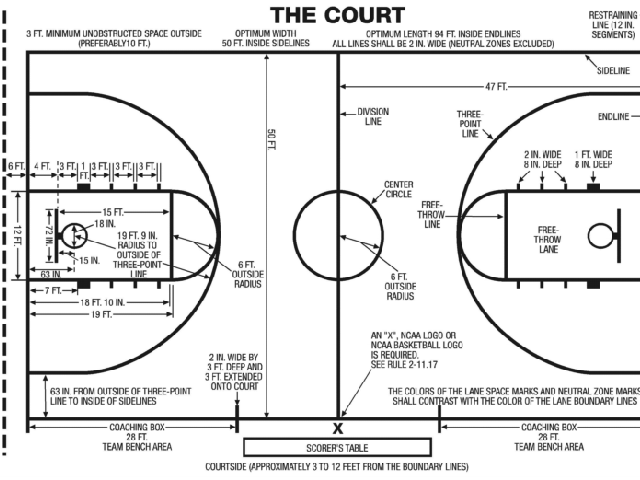
\includegraphics[width=14cm,height=8cm]{court.png}
\end{center}
\caption{Basketball Court}
\label{Img:court}
\end{figure}
\vspace{1cm}

%\textbf is used to make characters Bold.
\textbf{Basketball} is a sport played by two teams of five players on a rectangular court. The objective is to shoot a ball through a hoop 18 inches (46 cm) in diameter and 10 feet (3.0 m) high mounted to a backboard at each end. Basketball is one of the world\'s most popular and widely viewed sports.\\ % "\\" is used for newline.
A team can score a field goal by shooting the ball through the basket during regular play. A field goal scores two points for the shooting team if a player is touching or closer to the basket than the three-point line, and three points (known commonly as a 3 pointer or three) if the player is behind the three-point line. The team with the most points at the end of the game wins, but additional time (overtime) may be issued when the game ends with a draw. The ball can be advanced on the court by bouncing it while walking or running or throwing it to a team mate. It is a violation to move without dribbling the ball, to carry it, or to hold the ball with both hands then resume dribbling. 

\vspace{1cm}

\subsection{About NBA (National Basketball Association)}
\vspace{1cm}

\begin{figure}[ht]
\begin{center}

\includegraphics[width=1.5cm,height=2cm]{NBALogo.png}
\end{center}
\caption{NBA Logo}
\label{Img:NBALogo}
\end{figure}
\vspace{1cm}
The \textbf{National Basketball Association (NBA)} is the pre-eminent men\'s professional basketball league in North America, and is widely considered to be the premier men\'s professional basketball league in the world. It has 30 franchised member clubs (29 in the United States and 1 in Canada), and is an active member of USA Basketball (USAB), which is recognized by FIBA (also known as the International Basketball Federation) as the national governing body for basketball in the United States. The NBA is one of the four major North American professional sports leagues. NBA players are the world\'s best paid sportsmen, by average annual salary per player.
\vspace{1cm}

\subsection{About Chicago Bulls}
\vspace{1cm}
\begin{figure}[ht]
\begin{center}

\includegraphics[width=2cm,height=2cm]{ChiacgoBullsLogo.png}
\end{center}
\caption{Chicago Bulls Logo}
\label{Img:ChicagoBullsLogo}
\end{figure}
\vspace{1cm}
The \textbf{Chicago Bulls} are an American professional basketball team based in Chicago, Illinois, playing in the Central Division of the Eastern Conference in the National Basketball Association (NBA). The team was founded on January 26, 1966. The Bulls play their home games at the United Center, also known as the "Madhouse on Madison." The Bulls saw their greatest success during the 1990s. They are known for having one of the NBA\'s greatest dynasties, winning six NBA championships between 1991 and 1998 with two three-peats. All six championship teams were led by Hall of Famers Michael Jordan, Scottie Pippen and coach Phil Jackson. The Bulls are the only NBA franchise to win multiple championships and never lose an NBA Finals in their history.
\vspace{1cm}
\subsection{Interesting Facts about Chicago Bulls}

%This is used to create a numbered list.
\begin{enumerate}
\item They are known for having one of the NBA's greatest dynasties, winning six NBA championships between 1991 and 1998 with two three-peats.
\item The Bulls are the only NBA franchise to win multiple championships and never lose an NBA Finals in their history.
\item The Bulls won an NBA record-72 games during the 1995–-96 NBA season and are the only team in NBA history to win 70 games or more in a single season.
As of 2013, the Bulls were estimated to be the third most valuable NBA franchise according to Forbes, with an estimated value of \$1 billion, earning an estimated \$52.2 million in operating income in 2013.
\end{enumerate}
\vspace{1cm}

\section{Statistics in NBA}
Statistics in basketball are kept to evaluate a player or a team\'s performance.
Some statistics used are
%The following is used to create bullet points.
\begin{itemize}
\item PSG : Points Scored per Game for a Team
\item PAG : Points Scored Against per Game for a Team
\item Wins : Number of Wins for a Team
\item AST : Number of Assists made by the Team 
\end{itemize}
and so on..

%The \ref{Label} is used to reference a table in your rsweave document.
The section \ref{metaData} talks about it in depth.


\section{Reproducible Research}

\subsection{Code}
\subsubsection{Gathering the Data}

To install packages use the following command.

%eval=FALSE will not run the code in this chunk
\begin{Schunk}
\begin{Sinput}
> install.packages(c("Quandl","ggplot2","xtable"))
\end{Sinput}
\end{Schunk}

These are the packages being used. 

%options(width=80) -- sets the width of the box frame
\begin{Schunk}
\begin{Sinput}
> options(width=80)
> library(Quandl)
> library(ggplot2)
> library(xtable)
\end{Sinput}
\end{Schunk}

Getting the data from Quandl website using its API
To get the authcode you need to signup on the Quandl website which is free. After signing up you can find the Auth token in your Profile > Account Settings.

If we want to run a code chunk once and the output for when you compile the document again, rather than running the code chunk every time,set the option cache=TRUE.
When the chunk runs for the first time, the output is stored in a subdirectory called cache and the same is referred for all the later times, unless the chunk or its options are changed.

\begin{Schunk}
\begin{Sinput}
> bulls = Quandl("BBALL/NBA_CHICAGOBULLS",authcode="Jxdd68xhZxCpy3z-4ri9")
\end{Sinput}
\end{Schunk}

If you would like to generate a csv file for the raw data that we just fetched in your local workspace, use the following command :
\begin{Schunk}
\begin{Sinput}
> write.csv(bulls, file = "initialData.csv", row.names = FALSE)
\end{Sinput}
\end{Schunk}


Following command shows us the first few rows of the data
\begin{Schunk}
\begin{Sinput}
> head(bulls)
\end{Sinput}
\begin{Soutput}
        Year Wins Losses  W-L%   GB  PS/G  PA/G   SRS
1 2014-12-31   48     34 0.585  8.0  93.7  91.8  1.20
2 2013-12-31   45     37 0.549  4.5  93.2  92.9 -0.01
3 2012-12-31   50     16 0.758   NA  96.3  88.2  7.43
4 2011-12-31   62     20 0.756   NA  98.6  91.3  6.53
5 2010-12-31   41     41 0.500 20.0  97.5  99.1 -1.63
6 2009-12-31   41     41 0.500 25.0 102.2 102.5 -0.16
\end{Soutput}
\end{Schunk}


\subsubsection{Scrubbing the Data}

Manual examination reveals that we want all rows but not columns 3,4 and 5

\begin{Schunk}
\begin{Sinput}
> bulls.1 <- bulls[, -3:-5]
\end{Sinput}
\end{Schunk}

We still do not need the SRS column, hence removing it.
\begin{Schunk}
\begin{Sinput}
> bulls.final <- bulls.1 [, -5:-5]
\end{Sinput}
\end{Schunk}

Renaming the column names from PS/G , PA/G to PSG and PAG, respectively.

\begin{Schunk}
\begin{Sinput}
> colnames(bulls.final)[3] <- "PSG"
> colnames(bulls.final)[4] <- "PAG"
\end{Sinput}
\end{Schunk}

We run the below command to check the first few rows of our final data
\begin{Schunk}
\begin{Sinput}
> head(bulls.final)
\end{Sinput}
\begin{Soutput}
        Year Wins   PSG   PAG
1 2014-12-31   48  93.7  91.8
2 2013-12-31   45  93.2  92.9
3 2012-12-31   50  96.3  88.2
4 2011-12-31   62  98.6  91.3
5 2010-12-31   41  97.5  99.1
6 2009-12-31   41 102.2 102.5
\end{Soutput}
\end{Schunk}

Just in case you need this scrubbed data, use the following command to generate a csv file in your local workspace.
\begin{Schunk}
\begin{Sinput}
> write.csv(bulls.final, file = "finalData.csv", row.names = FALSE)
\end{Sinput}
\end{Schunk}


\vspace{1cm}
We will go through a list of commands to know more about the data that we have.

\subsection{Commands}
\subsubsection{Class()}

In every computer language variables provide a means of accessing the data stored in memory. R does not provide direct access to the computer\'s memory but rather provides a number of specialized data structures we will refer to as objects. These objects are referred to through symbols or variables. In R, however, the symbols are themselves objects and can be manipulated in the same way as any other object. This is different from many other languages and has wide ranging effects. 
The following data objects exist in R:

\begin{itemize}
\item Vectors
\item Lists
\item Arrays
\item Matrices
\item Tables
\item Data frames
\end{itemize}

We will now check the class of our final data object with the help of following command:

\begin{Schunk}
\begin{Sinput}
> class(bulls.final)
\end{Sinput}
\begin{Soutput}
[1] "data.frame"
\end{Soutput}
\end{Schunk}
Looking at the above result, we can conclude that the class of "bulls.final" that is an object which we have used to store our data is a Data frame.
  A data frame is a table, or two-dimensional array-like structure, in which each column contains measurements on one variable, and each row contains one case. As we shall see, a "case" is not necessarily the same as an experimental subject or unit, although they are often the same. Technically, in R a data frame is a list of column vectors, although there is only one reason why you might need to remember such an arcane thing. Unlike an array, the data you store in the columns of a data frame can be of various types. I.e., one column might be a numerical variable, another might be a factor, and a third might be a character variable. All columns have to be the same length (contain the same number of data items)

\subsubsection{Str()}
Compactly display the internal structure of an R object, a diagnostic function and an alternative to summary (and to some extent, dput). Ideally, only one line for each basic structure is displayed. It is especially well suited to compactly display the (abbreviated) contents of (possibly nested) lists. The idea is to give reasonable output for any R object. 
\begin{Schunk}
\begin{Sinput}
> str(bulls.final)
\end{Sinput}
\begin{Soutput}
'data.frame':	45 obs. of  4 variables:
 $ Year: Date, format: "2014-12-31" "2013-12-31" ...
 $ Wins: num  48 45 50 62 41 41 33 49 41 47 ...
 $ PSG : num  93.7 93.2 96.3 98.6 97.5 ...
 $ PAG : num  91.8 92.9 88.2 91.3 99.1 ...
\end{Soutput}
\end{Schunk}
Looking at the above result, it is quite clear that the first column is "Year" which is in "Date" format and has values like "2014-12-31".
  The second column is "Wins" which is a "numeric" field and has multiple values like 48,52 and so on.
  Likewise, we can understand the rest of the columns that are present in the data set.

\subsubsection{Summary()}
Summary is used to get a summary of a model object\'s contents.The Summary() command is is helpful for seeing the basic descriptive statistics for all the variables in a data frame and also the variables\' types. We use the following command to explore the summary of the data frame.
\begin{Schunk}
\begin{Sinput}
> options(width=80)
> summary(bulls.final)
\end{Sinput}
\begin{Soutput}
      Year                 Wins            PSG             PAG       
 Min.   :1970-12-31   Min.   :13.00   Min.   : 81.9   Min.   : 88.2  
 1st Qu.:1981-12-31   1st Qu.:31.00   1st Qu.: 96.7   1st Qu.: 94.9  
 Median :1992-12-31   Median :45.00   Median :102.2   Median : 99.1  
 Mean   :1992-12-30   Mean   :42.84   Mean   :101.2   Mean   :100.3  
 3rd Qu.:2003-12-31   3rd Qu.:51.00   3rd Qu.:106.6   3rd Qu.:105.0  
 Max.   :2014-12-31   Max.   :72.00   Max.   :114.9   Max.   :116.7  
\end{Soutput}
\end{Schunk}
Summary also shows a glimpse of statistics, including the mean, standard deviation, range, and percentiles of the values within the columns of a data set.
  
For example, lets consider the data present in "Wins" column. The minimum value for the data rows in the "Wins" is 13. The calculated Median for all the data rows of Wins is "45.0". The mean for all the data rows of Wins is "42.84"
\vspace{1cm}

\section{Results}
\subsection{Meta Data}

\begin{table}[h]
\begin{center}
\begin{tabular}{|l | l | l | l| }
\hline
Column Name & Data Type & Minimum Value & Maximum Value\\
\hline
Year & Date & 1900-01-01 & 2014-10-22\\
Wins & Number & 0 & 82\\
PSG & Number & 0 & NA\\
PAG & Number & 1 & NA\\
\hline
\end{tabular}
\end{center}
\caption{Metadata Information}
\label{metaTable}
\end{table}
\begin{description}
\item [Year] is a date column that can have values from 1st January 1900 to 31st December 2014.
\item [Wins], that is a numeric value can have any values between 0 and 82. The maximum number of games that a NBA team can play in a year is 82 and hence, highest possible number of wins can be 82.
\item [PSG] i.e nothing but points scored by Chicago bulls in an year, that is a numeric field can have values from 0 to 150. It is calculated by dividing the total number of points(team) by number of games(team). 
\item [PAG] i.e nothing but points scored against Chicago bulls in an year, that is a numeric field can have values from 0 to 150. It is calculated by dividing the total number of points against(team) by number of games(team). 
\end{description}

\subsection{Data Set}

Table \ref{dataTable} shows how the data looks like that we have gathered and cleaned. 
We have collected Data starting from the year 1970 to 2014. 
Chicago Bulls had the highest number of wins in the year 1972, whereas 1999 being the worst performance year for them. The data also shows decrease in the number of points scored per game after 1997. Moreover, the number of points scored against the Chicago Bulls have reduced gradually.

%[H] - is used to place the table "Here".
\begin{table}[H]
\centering
% latex table generated in R 3.1.1 by xtable 1.7-4 package
% Tue Oct 21 23:09:51 2014
\begin{tabular}{| c | c | c | c|}
  \hline
Year & Wins & PSG & PAG \\ 
  \hline
2014-12-31 & 48 & 93.70 & 91.80 \\ 
  2013-12-31 & 45 & 93.20 & 92.90 \\ 
  2012-12-31 & 50 & 96.30 & 88.20 \\ 
  2011-12-31 & 62 & 98.60 & 91.30 \\ 
  2010-12-31 & 41 & 97.50 & 99.10 \\ 
  2009-12-31 & 41 & 102.20 & 102.50 \\ 
  2008-12-31 & 33 & 97.30 & 100.40 \\ 
  2007-12-31 & 49 & 98.80 & 93.80 \\ 
  2006-12-31 & 41 & 97.80 & 97.20 \\ 
  2005-12-31 & 47 & 94.50 & 93.40 \\ 
  2004-12-31 & 23 & 89.70 & 96.00 \\ 
  2003-12-31 & 30 & 95.00 & 100.10 \\ 
  2002-12-31 & 21 & 89.50 & 98.00 \\ 
  2001-12-31 & 15 & 87.60 & 96.70 \\ 
  2000-12-31 & 17 & 84.80 & 94.20 \\ 
  1999-12-31 & 13 & 81.90 & 91.40 \\ 
  1998-12-31 & 62 & 96.70 & 89.60 \\ 
  1997-12-31 & 69 & 103.10 & 92.30 \\ 
  1996-12-31 & 72 & 105.20 & 92.90 \\ 
  1995-12-31 & 47 & 101.50 & 96.70 \\ 
  1994-12-31 & 55 & 98.00 & 94.90 \\ 
  1993-12-31 & 57 & 105.20 & 98.90 \\ 
  1992-12-31 & 67 & 109.90 & 99.50 \\ 
  1991-12-31 & 61 & 110.00 & 101.00 \\ 
  1990-12-31 & 55 & 109.50 & 106.20 \\ 
  1989-12-31 & 47 & 106.40 & 105.00 \\ 
  1988-12-31 & 50 & 105.00 & 101.60 \\ 
  1987-12-31 & 40 & 104.80 & 103.90 \\ 
  1986-12-31 & 30 & 109.30 & 113.10 \\ 
  1985-12-31 & 38 & 108.70 & 109.60 \\ 
  1984-12-31 & 27 & 103.70 & 108.90 \\ 
  1983-12-31 & 28 & 111.00 & 115.90 \\ 
  1982-12-31 & 34 & 106.60 & 108.60 \\ 
  1981-12-31 & 45 & 109.00 & 107.00 \\ 
  1980-12-31 & 30 & 107.50 & 110.20 \\ 
  1979-12-31 & 31 & 104.70 & 108.70 \\ 
  1978-12-31 & 40 & 103.90 & 104.80 \\ 
  1977-12-31 & 44 & 98.90 & 98.00 \\ 
  1976-12-31 & 24 & 95.90 & 98.80 \\ 
  1975-12-31 & 47 & 98.10 & 95.00 \\ 
  1974-12-31 & 54 & 102.00 & 98.70 \\ 
  1973-12-31 & 51 & 104.10 & 100.60 \\ 
  1972-12-31 & 57 & 111.20 & 102.90 \\ 
  1971-12-31 & 51 & 110.60 & 105.40 \\ 
  1970-12-31 & 39 & 114.90 & 116.70 \\ 
   \hline
\end{tabular}\caption{Data set for Chicago Bulls}
\label{dataTable}
\end{table}





\subsection{Graph}
\begin{figure}[H]

Following command is used to plot a line graph based on the data that we have.
As the legend clearly states, we have three distinct lines showing Number of wins, Points scored per game by the Bulls team and lastly points scored against the Bulls team per game.

\begin{Schunk}
\begin{Sinput}
> ggplot(data=bulls.final, aes(x=Year)) + ylab("")+
+   geom_line(aes(y = Wins, colour = "Wins")) + 
+   geom_line(aes(y = PSG, colour = "Points Scored/Game"),size=0.5)+
+   geom_line(aes(y = PAG, colour = "Points Against/Game"),size=0.5) +
+   #ggtitle("Performance of Chicago Bulls") +   # Set title
+   scale_colour_hue(name="Legend ") # Renaming the Title of legend
\end{Sinput}
\end{Schunk}
\includegraphics{Assignment2-chunk11}
\caption{Performance of Chicago Bulls}
\label{PerChicagoBullsLogo}
\end{figure}


\paragraph
The graph in Figure \ref{PerChicagoBullsLogo} tells us about the performance of Chicago Bulls.
\\
The list below summarizes the history of Chicago Bulls\\
1966--1974: Early success.\\
1976--1984: Gilmore and Theus.\\
1984--1998: The Michael Jordan Era.\\
1999--2004: Rebuilding.\\
2004--2007: Resurgence.\\
2007--2008: Missing the playoffs.\\
2008--present: The Derrick Rose era.\\
\\
It is certainly evident that there was a steep fall in the number of wins during 1998-2000. However, as the summary above states this is when the Chicago Bulls were in the rebuilding phase and later came the Resurgence period, where the team came back to winning.\\
\\
The Chicago Bulls joined the NBA for the 1966-67 season. The franchise struggled for the better part of a quarter century, occasionally putting excellent teams on the court, such as the tough units of the mid-1970s that featured Bob Love, Norm Van Lier, Jerry Sloan, and Tom Boerwinkle. More often, however, the Bulls worked hard for mediocre results. That all changed in the mid-1980s with the drafting of Michael Jordan, the dominant player of his era and possibly the greatest player of all time.\\
\\
Jordan won seven straight scoring titles with a combination of breathtaking slam dunks and a bag of thrilling shot-making tricks. He put up some of the biggest numbers in NBA history and wrote some of the most memorable chapters in the annals of the league. The addition of Scottie Pippen, another Hall of Famer, in 1987 would set the stage for one of sport\'s great dynasties.\\
\\
In the early 1990s, the Bulls assembled a strong supporting cast for Jordan and Pippen which won three consecutive NBA titles, becoming only the third franchise in history to string together a trio of crowns. After more than a year of "retirement" to try his hand at professional baseball, Jordan returned to lead the Bulls back to another title in 1996, one more in 1997 and a third in a row in 1998, the Bulls\'  second three-peat of the decade and their sixth NBA championship trophy.\\
\\
Ten years later, Chicago beat overwhelming odds to win the NBA Draft Lottery, meaning the Bulls had the top pick in the 2008 NBA Draft. Point guard Derrick Rose was the team\'s choice, and he has since led the Bulls to the playoffs in each of his professional campaigns, including a trip to the 2011 Eastern Conference Finals.\\

\centering
 THE END 
\end{document}


